% ##################################################################################################################
\section{Poznan}
\label{sec:poznan}
\hfill \textbf{Author:} Michal Maciejewski, Waldemar Walerjanczyk

% ##################################################################################################################
\mm{Add WW to the book contributors}
\ah{Done. Could you please shortly check for errors? Thx.}

% ##################################################################################################################
Poznan, with its population of over 550\,000, is the fifth largest city in Poland, and together with the neighboring suburban area, it makes up an agglomeration inhabited by nearly one million people. The development of the MATSim scenario for the Poznan agglomeration began in 2012, and since then, the model has been continuously extended and improved. Currently, it is a 24-hour microscopic model of private transport. The goal is to create a 24-hour multi-agent activity-based simulation of the Poznan agglomeration, combining both private and public transport.

The road network model was extracted from \gls{osm} and includes all roads and link roads (such as entrances or exits from motorways). The final result is a high-detail road network model that consists of 17\,026 nodes and 40\,129 links. This model was calibrated in order to determine traffic flow parameters for links (e.g.,\,flow capacity, storage capacity, free-flow speed) for each of the 13\,modeled road classes. \mm{ref to the OSM paper by BP and MM}

The travel demand model was derived from the official trip-based 4-stage model used by the planning department of the city of Poznan; this model dates back to 2000 but since then has been frequently updated. Since the official model was originally designed for the the morning and afternoon peak hours, it had to be extended to describe travel demand throughout the day, hour after hour. As a result, the demand for private transport is represented by 24\,sets of hourly \gls{od} matrices, each set consisting of nine different matrices, one for each of nine travel motivations, namely home $\rightarrow$ work/education/shopping/other, work/education/shopping/other $\rightarrow$ home, and not related to home. This totals up to 216\,\gls{od} matrices. \mm{ref to the SysTrans paper by MM, BP, WW and AS; and to Przeglad Komunikacyjny??}

The official model divides the agglomeration into 417\,zones \mm{Waldek, ile bylo faktycznie zon, a ile to zony zewnetrzne?}, which is not sufficient for the activity locations to be accurately modeled at the microscopic level. To increase the accuracy, the \gls{osm} land use data were used.

Six types of land use, namely residential, industrial, green, commercial, schools and unclassified, were used to subdivide zones into homogenous subzones. As a result, home activities were located in residential subzones, education activities at schools, shopping in residential or commercial subzones, and so on. Figure~\ref{fig:poznan_home_distribution} illustrates the distribution of \emph{home} locations when land use is taken into account. \mm{ref to the GIS paper by BP and MM}

%---------------------------------------------------------------------
\createfigure%
{Distribution of home activities based on land use}%
{Distribution of home activities based on land use}%
{\label{fig:poznan_home_distribution}}%
{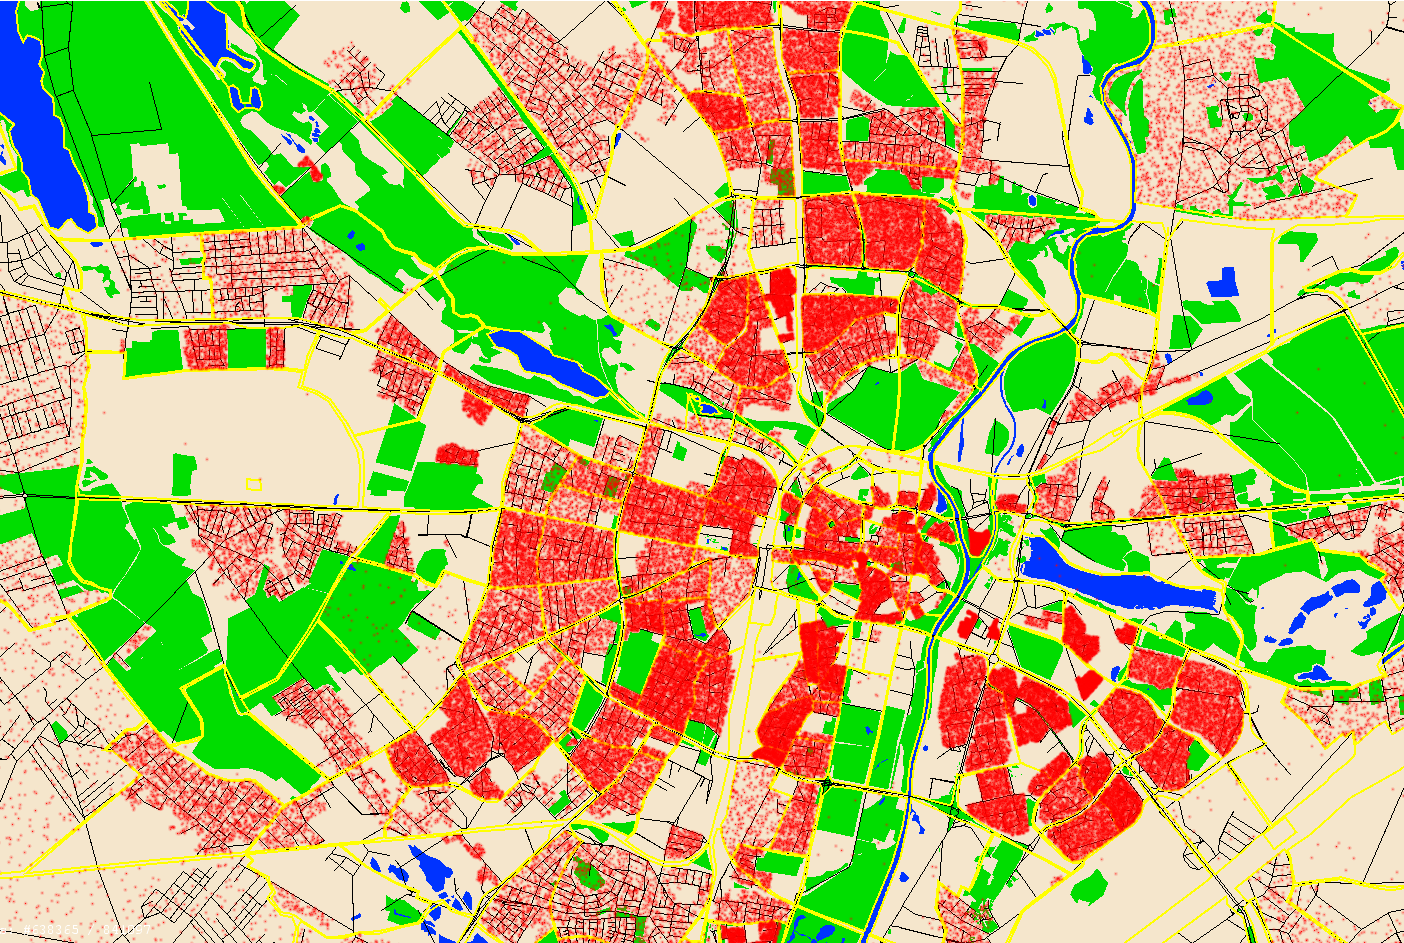
\includegraphics[width=\textwidth, angle=0]{using/figures/poznan_home_distribution}}%
{}%
%---------------------------------------------------------------------

Having calculated the \gls{od} matrices for private transport and subdivided the area into homogenous subzones, the next step was to generate the population of agents. In the first attempt, an assumption was made that each agent performs only one trip, so the number of agents equals the demand represented by the \gls{od} matrices, which is almost 840\,000. Departure times were randomly distributed (uniform distribution) over each hour hour, and therefore, the only decision made by each agent during the replanning phase concerned the route choice for the preselected pair of locations. The whole simulation takes 120\,iterations, but the relaxed state is usually achieved after 60\,iterations. Figure~\ref{fig:poznan_traffic_simulation} shows the state of traffic at 7:00\,am.

%---------------------------------------------------------------------
\createfigure%
{Road traffic in the Poznan agglomeration at 7:00\,am}%
{Road traffic in the Poznan agglomeration at 7:00\,am}%
{\label{fig:poznan_traffic_simulation}}%
{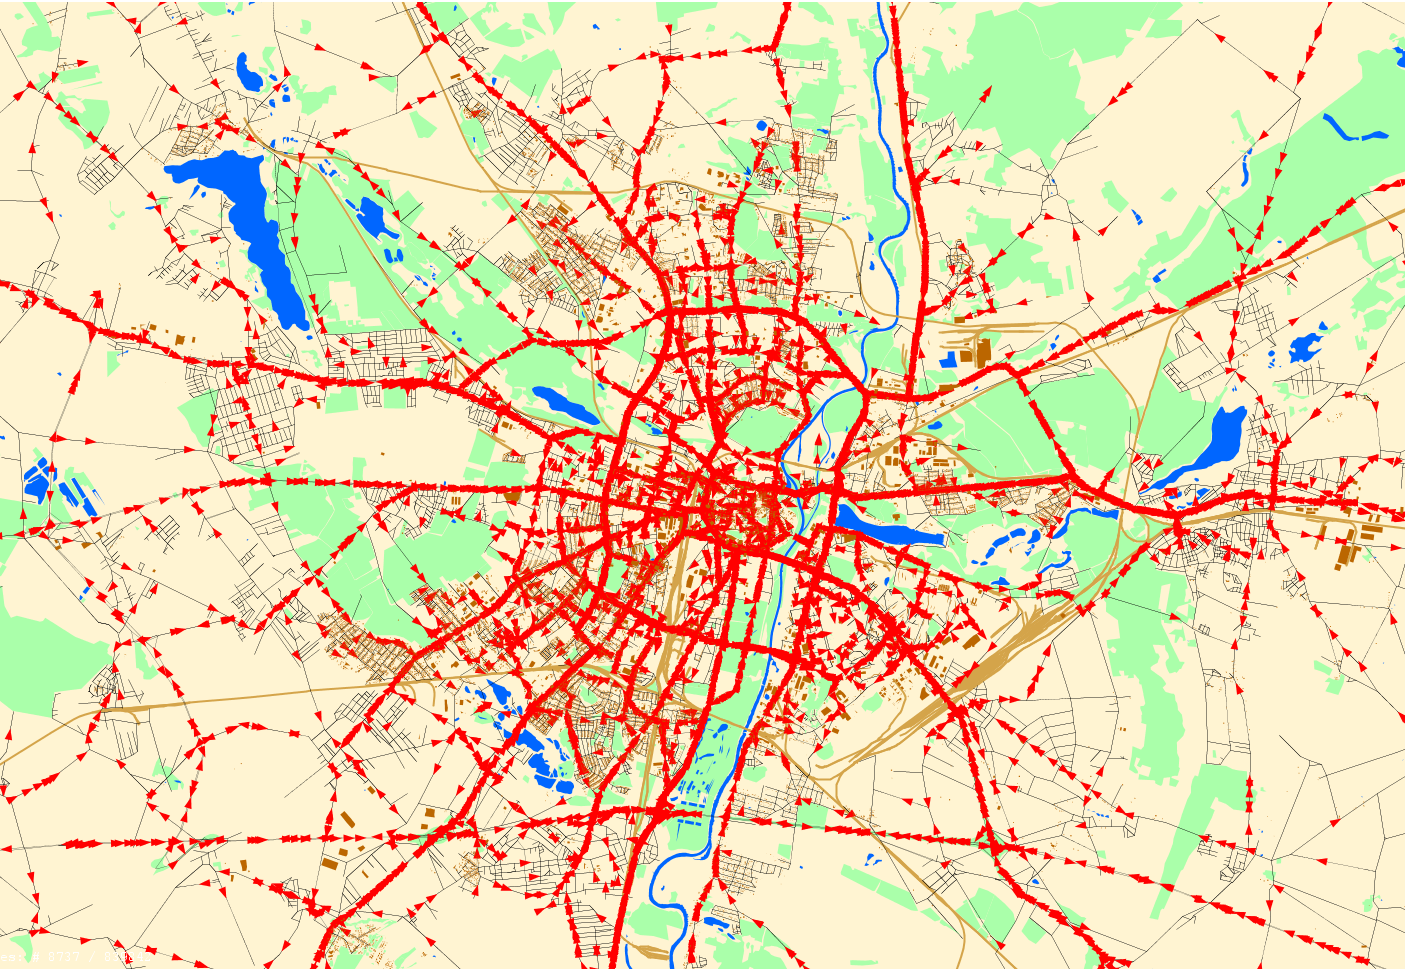
\includegraphics[width=\textwidth, angle=0]{using/figures/poznan_traffic_simulation}}%
{}%
%---------------------------------------------------------------------

Currently, the model is being updated according to the Comprehensive Travel Study carried out in 2014. At the same time, the public transport system is being added, hence allowing for simulating both private and public transport. The Poznan model has been used for simulation of real-time electric taxi dispatching, which is done by means of the DVRP extension \mm{ref to some taxi papers?}.

% ##################################################################################################################